\documentclass{article}

\usepackage[inline]{enumitem}
\usepackage{graphicx}

\begin{document}
\noindent{}\rule{\textwidth}{0.4pt}
\begin{center}
	\'{A}lgebra Linear\\
	Lista 2 --- Vetores e equa\c{c}\~oes da reta e do plano \\
	\vspace{0.2cm}
	Prof. Adriano Barbosa
\end{center}
\noindent{}\rule{\textwidth}{0.4pt}

\begin{enumerate}
%%%%%%%%%%%%%%%%%%%%%%%%%%%%%%%%%%%%%%%%%%%%%
\item Decida se as afirma\c{c}\~oes s\~ao verdadeiras ou falsas:

\begin{enumerate}
	\item Se $u = v$, ent\~ao $\|u\| = \|v\|$.
	\item Se $\|u\| = \|v\|$, ent\~ao $u = v$.
	\item Se $u$ \'e paralelo a $v$, ent\~ao $u = v$.
	\item Se $u = v$, ent\~ao $u$ \'e paralelo a $v$.
	\item Se $w = u + v$, ent\~ao $\|w\| = \|u\| + \|v\|$.
	\item $\|w\| = \|u\| + \|v\|$, ent\~ao $u$, $v$ e $w$ s\~ao paralelos.
	\item $\|5v\| = \|-5v\| = 5\|v\|$.
	\item Os vetores $3v$ e $-4v$ s\~ao paralelos e de mesmo sentido.
	\item Se $u$ \'e paralelo a $v$, $\|u\| = 2$ e $\|v\| = 4$, ent\~ao $v = 2u$ ou $v = -2u$.
\end{enumerate}

%%%%%%%%%%%%%%%%%%%%%%%%%%%%%%%%%%%%%%%%%%%%%
\item Dados tr\^es pontos $A$, $B$ e $C$, represente graficamente os segmentos orientados

\begin{minipage}{0.4\textwidth}
	\begin{enumerate}
		\item $BA + 2 BC$
		\item $2 CA + 2 BA$
		\item $3 AB - 2 BC$
		\item $\frac{1}{2} AB - 2 CB$
	\end{enumerate}
\end{minipage}
\begin{minipage}{0.4\textwidth}
	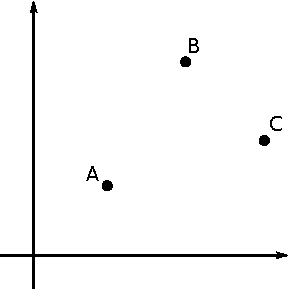
\includegraphics[scale=0.6]{plano.pdf}
\end{minipage}

%%%%%%%%%%%%%%%%%%%%%%%%%%%%%%%%%%%%%%%%%%%%%
\item Escreva as equa\c{c}\~oes param\'etricas das retas que passam por

\begin{minipage}{0.4\textwidth}
	\begin{enumerate}
		\item A e B
		\item C e D
		\item B e C
		\item D e E
	\end{enumerate}
\end{minipage}
\begin{minipage}{0.4\textwidth}
	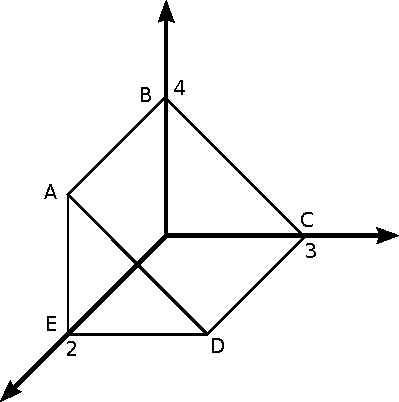
\includegraphics[scale=0.6]{piramide.pdf}
\end{minipage}

%%%%%%%%%%%%%%%%%%%%%%%%%%%%%%%%%%%%%%%%%%%%%
\item Determine a equa\c{c}\~ao param\'etrica da reta $r$ definida pelos pontos $A = (2, -3, 4)$ e $B = (1, -1, 2)$ e verifique se os pontos $C = (\frac{5}{2}, -4, 5)$ e $D = (-1, 3, 4)$ pertencem a $r$.

%%%%%%%%%%%%%%%%%%%%%%%%%%%%%%%%%%%%%%%%%%%%%
\item Escreva a equa\c{c}\~ao param\'etrica da reta que passa por $A = (1, 2, 3)$ e \'e paralela a reta $r: (x, y, z) = (1, 4, 3) + t(0, 0, 1)$

%%%%%%%%%%%%%%%%%%%%%%%%%%%%%%%%%%%%%%%%%%%%%
\item Verifique se os pontos $P_1 = (5, -5, 6)$ e $P_2 = (4, -1, 12)$ pertencem a reta $\displaystyle r: -(x-3) = \frac{y+1}{2} = -\frac{z-2}{2}$

%%%%%%%%%%%%%%%%%%%%%%%%%%%%%%%%%%%%%%%%%%%%%
% \item Represente graficamente as retas de equa\c{c}\~oes

% \begin{enumerate}
% 	\item $x = y = z$
% 	\item 
% 		$\left\{\begin{array}{l}
% 			y = -x \\
% 			z = 3 + x
% 		\end{array}\right.$
% 	\item 
% 		$\left\{\begin{array}{l}
% 			x = 1 - t \\
% 			y = -1 + 2t \\
% 			z = 2 + t
% 		\end{array}\right.$
% 	\item 
% 		$\left\{\begin{array}{l}
% 			y = 2x \\
% 			z = 3
% 		\end{array}\right.$
% \end{enumerate}

%%%%%%%%%%%%%%%%%%%%%%%%%%%%%%%%%%%%%%%%%%%%%
\item Determine o \^angulo entre as retas

\begin{enumerate}
	\item
		$r_1:\left\{\begin{array}{l}
			x = -2 -t \\
			y = t \\
			z = 3 - 2t
		\end{array}\right.$
	\ \ \ \ \ e\ \ \ \ \ 
		$r_2:\begin{array}{l}
			\frac{x}{2} = y+6 = z-1
		\end{array}$
	\item
		$r_1:\left\{\begin{array}{l}
			x = 1 + \sqrt{2}t \\
			y = t \\
			z = 5 - 3t
		\end{array}\right.$
	\ \ \ \ \ e\ \ \ \ \ 
		$r_2:\left\{\begin{array}{l}
			x = 3 \\
			y = 2
		\end{array}\right.$
\end{enumerate}

%%%%%%%%%%%%%%%%%%%%%%%%%%%%%%%%%%%%%%%%%%%%%
\item Determine o valor de $n$ para que o \^angulo entre as retas seja $\frac{\pi}{6}$

$r_1:\begin{array}{l}
	\frac{x-2}{4} = \frac{y}{5} = \frac{z}{3}
\end{array}$
\ \ \ \ \ e\ \ \ \ \ 
$r_2:\left\{\begin{array}{l}
	y = nx + 5 \\
	z = 2x - 2
\end{array}\right.$

%%%%%%%%%%%%%%%%%%%%%%%%%%%%%%%%%%%%%%%%%%%%%
\item Dados $A = (3, 4, -2)$ e 
$r:\left\{\begin{array}{l}
	x = 1 + t \\
	y = 2 - t \\
	z = 4 + 2t
\end{array}\right.$. Determine a equa\c{c}\~ao param\'etrica da reta que passa por $A$ e \'e perpendicular a $r$.

%%%%%%%%%%%%%%%%%%%%%%%%%%%%%%%%%%%%%%%%%%%%%
\item Encontre a reta que passa pelo ponto m\'edio do segmento de extremos $A = (5, -1, 4)$ e $B = (-1, -7, 1)$ e seja perpendicular a ele.

%%%%%%%%%%%%%%%%%%%%%%%%%%%%%%%%%%%%%%%%%%%%%
\item Seja o plano $\pi: 3x + y -z = 4$, calcule:

\begin{enumerate}
	\item O ponto de $\pi$ que tem coordenadas $x=1$ e $y=3$;
	\item O ponto de $\pi$ que tem coordenadas $x=0$ e $z=2$;
	\item O valor de $k$ para que o ponto $P = (k, 2, k-1)$ perten\c{c}a a $\pi$;
	\item O ponto de coordenada $x=2$ cuja coordenada $y$ \'e o dobro da coordenada $z$;
	\item O valor de $k$ para que o plano $\pi_1:kx-4y+4z = 7$ seja paralelo a $\pi$.
\end{enumerate}

%%%%%%%%%%%%%%%%%%%%%%%%%%%%%%%%%%%%%%%%%%%%%
\item Dada a equa\c{c}\~ao geral do plano $\pi: 3x - 2y - z = 6$, encontre as equa\c{c}\~oes param\'etricas de $\pi$.

%%%%%%%%%%%%%%%%%%%%%%%%%%%%%%%%%%%%%%%%%%%%%
\item Encontre a equa\c{c}\~ao geral do plano 
$\left\{\begin{array}{l}
	x = 1 + h - 2t \\
	y = 1 - t \\
	z = 4 + 2h - 2t
\end{array}\right.$

%%%%%%%%%%%%%%%%%%%%%%%%%%%%%%%%%%%%%%%%%%%%%
\item Encontre a equa\c{c}\~ao geral do plano que cont\'em as retas

\begin{enumerate}
	\item
		$r_1:\left\{\begin{array}{l}
			y = 2x - 3 \\
			z = -x + 2
		\end{array}\right.$
	\ \ \ \ \ e\ \ \ \ \ 
		$r_2:\left\{\begin{array}{l}
			\frac{x-1}{3} = z-1 \\
			y = -1
		\end{array}\right.$
	\item
		$r_1:\left\{\begin{array}{l}
			x = 1 + 2t \\
			y = -2 + 3t \\
			z = 3 -t
		\end{array}\right.$
	\ \ \ \ \ e\ \ \ \ \ 
		$r_2:\left\{\begin{array}{l}
			x = 1 - 2t \\
			y = -2 - t \\
			z = 3 + 2t
		\end{array}\right.$
\end{enumerate}

%%%%%%%%%%%%%%%%%%%%%%%%%%%%%%%%%%%%%%%%%%%%%
\item Determine a equa\c{c}\~ao geral do plano que cont\'em

\begin{enumerate}
	\item o ponto $A = (4, 3, 2)$ e a reta
		$r:\left\{\begin{array}{l}
			x = t \\
			y = 2 -t \\
			z = 3 + 2t
		\end{array}\right.$

	\item o ponto $A = (1, -1, 2)$ e o eixo $z$
\end{enumerate}

%%%%%%%%%%%%%%%%%%%%%%%%%%%%%%%%%%%%%%%%%%%%%
\item Verifique se a reta $r$ est\'a contida no plano $\pi$

\begin{enumerate}
	\item 
		$r:\left\{\begin{array}{l}
			y = 4x + 1 \\
			z = 2x - 1
		\end{array}\right.$
	\ \ \ \ \ e\ \ \ \ \ 
		$\pi:2x + y - 3z - 4 = 0$
	
	\item
		$r: x-2 = \frac{y+2}{2} = z+3$
	\ \ \ \ \ e\ \ \ \ \ 
		$\pi:\left\{\begin{array}{l}
			x = h + t \\
			y = -1 + 2h - 3t \\
			z = -3 + h -t
		\end{array}\right.$

\end{enumerate}

%%%%%%%%%%%%%%%%%%%%%%%%%%%%%%%%%%%%%%%%%%%%%
\item Encontre a equa\c{c}\~ao param\'etrica do plano paralelo ao eixo dos $z$ e que intercepta o eixo dos $x$ em $-3$ e dos $y$ em $4$.

%%%%%%%%%%%%%%%%%%%%%%%%%%%%%%%%%%%%%%%%%%%%%
\item Encontre a equa\c{c}\~ao param\'etrica do plano paralelo ao plano $xz$ e que intercpta o eixo dos $y$ em $-7$.

\end{enumerate}
\end{document}
